\documentclass[titlepage]{article}
\usepackage{graphicx}
\usepackage{listings}
\usepackage{color}
\usepackage[dvipsnames]{xcolor}
\usepackage{gensymb}
\usepackage[linguistics]{forest}
\usepackage{amsmath}
\usepackage{listings}
\usepackage{tikz}
\usetikzlibrary{mindmap}
\pagestyle{empty}

\definecolor{dkgreen}{rgb}{0,0.6,0}
\definecolor{gray}{rgb}{0.5,0.5,0.5}
\definecolor{mauve}{rgb}{0.58,0,0.82}
\definecolor{magenta}{HTML}{F10088}
\definecolor{plum}{HTML}{95298A}
\definecolor{tan}{HTML}{DC9C7B}
\definecolor{aquamarine}{HTML}{00B5BC}
\makeatletter
\setlength{\@fptop}{0pt}
\makeatother

\makeatletter
\newcommand*{\rom}[1]{\expandafter\@slowromancap\romannumeral #1@}
\makeatother

\lstset{frame=tb,
  language=Java,
  aboveskip=3mm,
  belowskip=3mm,
  showstringspaces=false,
  columns=flexible,
  basicstyle={\small\ttfamily},
  numbers=none,
  numberstyle=\tiny\color{gray},
  keywordstyle=\color{blue},
  commentstyle=\color{dkgreen},
  stringstyle=\color{mauve},
  breaklines=true,
  breakatwhitespace=true,
  tabsize=3
}

\title{ECE408 - Applied Parallel Programming \\ Final Report}
\author{Neil Singh (ngsingh2) \\ Patrick McMahon (pfmcmah2) \\ Matthew Krikorian (krikorn2)}

\begin{document}

\maketitle

\section*{Milestone 1}
Milestone 1 of this project was mostly setting up our test environment and preparing it to start developing the later parts of this project. 

\subsection*{Running Time of m1.1.py}
For m1.1.py, we had an accuracy of 0.8673, and an elapsed running time of 9.76 seconds.

\subsection*{Running Time of m1.2.py}
For m1.2.py, we had an accuracy of 0.8673, and an elapsed running time of 3.19 seconds.

\subsection*{Most Time Consuming Kernels}
Some of the most time consuming kernels when running the nvprof profile were the\textit{implicit\_convolve\_sgemm} kernel, taking up 36.96\% of the execution time, the \textit{activation\_fw\_4d\_kernel} kernel, taking up 14.33\% of the execution time, and the \textit{pooling\_fw\_4d\_kernel} kernel, which took up 10.69\% of the programs execution time.

\newpage

\section*{Milestone 2}
In this milestone of the project, we were tasked with writing sequential convolution code. Using the skeleton from our textbook, and the corresponding data accesses, we successfully implemented the function below.

\begin{figure}[h!]
\begin{lstlisting}[language=C++]
{
    const int B = x.shape_[0];
    const int M = y.shape_[1];
    const int C = x.shape_[1];
    const int H = x.shape_[2];
    const int W = x.shape_[3];
    const int K = k.shape_[3];

    int H_out = H - K + 1;
    int W_out = W - K + 1;

    for (int b = 0; b < B; ++b)
    {
      for (int m = 0; m < M; m++)
      {
        for (int h = 0; h < H_out; h++)
        {
          for (int w = 0; w < W_out; w++)
          {
            y[b][m][h][w] = 0;

            for (int c = 0; c < C; c++)
            {
              for (int p = 0; p < K; p++)
              {
                for (int q = 0; q < K; q++)
                {
                  y[b][m][h][w] += x[b][c][h + p][w + q] * k[m][c][p][q];
                }
              }
            }
          }
        }
      }
    }
}
\end{lstlisting}
\caption{Our CPU implementation of the convolutional layer in MxNet}
\end{figure}

\newpage

\subsection*{Our Results For Respective Models}

\begin{figure}[h!]
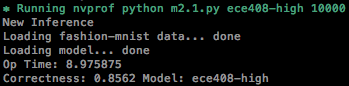
\includegraphics[width=\linewidth]{ece-408-high-10000.png}
\caption{Accuracy and elapsed time for high correctness and sample size 10000}
\label{fig:flowFree}
\end{figure}

\begin{figure}[h!]
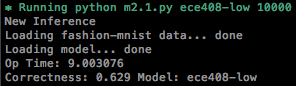
\includegraphics[width=\linewidth]{ece-408-low-10000.png}
\caption{Accuracy and elapsed time for low correctness and sample size 10000}
\label{fig:flowFree}
\end{figure}

\newpage
\section*{Milestone 3}
In this milestone we were tasked with writing a baseline paralllel convolution kernel that had to pass several baseline tests. This implementation is very sub-optimal, as it uses a TILE\_WIDTH of 1.
\begin{figure}[h!]
\begin{lstlisting}[language=C++]
{
    const int H_out = H - K + 1;
    const int W_out = W - K + 1;
    
    #define y4d(i3,i2,i1,i0) y[(i3) * (M * H_out * W_out) + (i2)*(H_out * W_out) + (i1)*(W_out) + i0]
    #define x4d(i3,i2,i1,i0) x[(i3) * (C * H * W) + (i2)*(H * W) + (i1)*(W) + i0]
    #define k4d(i3,i2,i1,i0) k[(i3) * (C * K * K) + (i2)*(K * K) + (i1)*(K) + i0]

    int W_grid = ceil(W_out / (float)TILE_WIDTH);
    int H_grid = ceil(H_out / (float)TILE_WIDTH);
    int n, m, h, w, c, p, q;
    n = blockIdx.x;
    m = blockIdx.y;
    h = blockIdx.z / W_grid + threadIdx.y;
    w = blockIdx.z % W_grid + threadIdx.x;
    
    float acc = 0;
    for (c = 0; c < C; c++) {
        for (p = 0; p < K; p++) {
            for (q = 0; q < K; q++) {
                if (h+p < H && w+q < W)
                    acc += x4d(n, c, h+p, w+q) * k4d(m, c, p, q);
            }
        }
    }
    y4d(n, m, h, w) = acc;

    #undef y4d
    #undef x4d
    #undef k4d
}
\end{lstlisting}
\caption{Our GPU implementation of the convolutional layer in MxNet}
\end{figure}

\newpage
\subsection*{Nvprof GPU Profile}
\begin{figure}[h!]
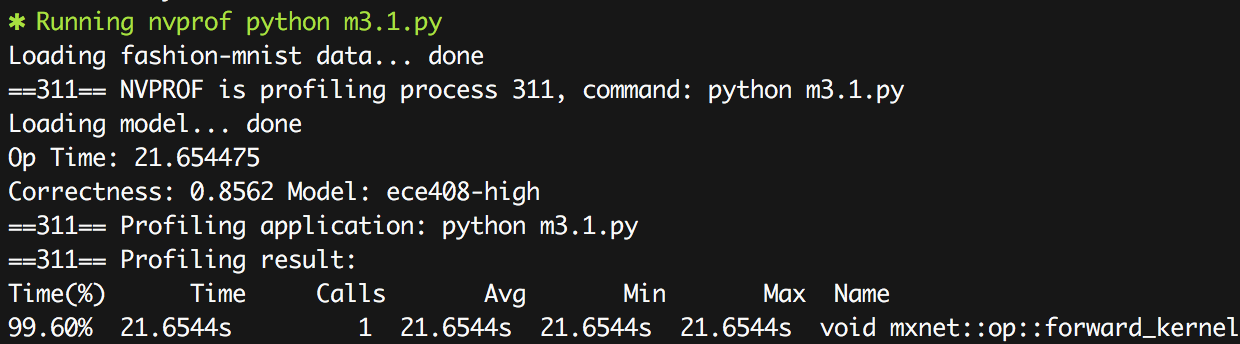
\includegraphics[width=\linewidth]{nvprof.png}
\caption{Nvprof GPU profile for our forward kernel}
\label{fig:flowFree}
\end{figure}

\newpage

\section*{Optimized Layer}

\subsection*{Initial Optimization}
We knew right off the bat that the first thing we were going to need to optimize was the way our implementation handled tiling. Our current implementation was giving us a slightly incorrect accuracy for any TILE\_SIZE above 1, so we first had to correct that to speedup our kernel. Below is the corrected kernel from part 2, which led to an average Op time of about 450ms instead of the 14s we got with our implementation where TILE\_SIZE = 1. This new implementation had TILE\_SIZE = 8. This was due in part to the correction of all the floating point operations we had.


\begin{figure}[h!]
\begin{lstlisting}[language=C++]
{
    int W_grid = (int) ceil(W_out / TILE_WIDTH * 1.0);
//  int H_grid = ceil(H_out / TILE_WIDTH * 1.0);
    int n, m, h, w, c, p, q;
    n = blockIdx.x;
    m = blockIdx.y;
    h = (blockIdx.z / W_grid) * TILE_WIDTH + threadIdx.y;
    w = (blockIdx.z % W_grid) * TILE_WIDTH + threadIdx.x;
    float acc = 0.0;
    for (c = 0; c < C; c++) {
      for (p = 0; p < K; p++) {
        for (q = 0; q < K; q++) {
//        if (h+p < H && w+q < W)
            acc += x4d(n, c, h+p, w+q) * k4d(m, c, p, q);
          }
        }
    }
    y4d(n, m, h, w) = acc;}
\end{lstlisting}
\caption{Our first improved GPU implementation with TILE\_SIZE = 8}
\end{figure}

\newpage
\subsection*{Further Optimization}
After we made this initial optimization, we knew that a running time of about 450ms was still too poor to really say we made any real optimizations to the kernel. After this point, we chose to optimize the shared memory and tiling implementation of our kernel, to improve on the DRAM accesses our code was making. Rather than taking variables from shared memory, our implementation was making calls to global memory every time it wanted to make an operation, which is highly inefficient. To correct this, we allocated shared memory for both the inputs and the weight matrix, to allow for much faster accesses to speed up our implementation. In our new implementation, we load the filter W into shared memory, then all the threads work together to load the input into a shared memory array. Then part of the sum is computed and put into Y, and then the calculation moves onto the next channel where the threads perform the next subset of convolution. We thought this optimization would be fruitful because we were now going to use shared memory to handle our operations, which would severely decrease our running time by reducing the latency to global memory accesses. With this new and improved implementation, we were able to reduce our running time all the way down to 151ms (200ms when we run Nvprof). Below is our implementation.

\newpage

\subsection*{Optimization Code}
\begin{figure}[h!]
\begin{lstlisting}[language=C++]
for(c = 0; c < C; c++)
    {
      if((h0 < K) && (w0 < K))
      {
        W_shared[h0*K+w0] = k4d(m, c, h0, w0);
      }

      //__syncthreads();

      int itemp = h0temp;
      for(i = h; i < h_base + X_tile_width; i += TILE_WIDTH, itemp += x_tile_tile_width)
      {
        for(j = w; j < w_base + X_tile_width; j += TILE_WIDTH)
        {
            X_shared[itemp + (j - w_base)] = x4d(n, c, i, j);
        }
      }

      __syncthreads();

      int ptemp = h0temp;
      for(p = 0; p < k2; p += K, ptemp += X_tile_width)
      {
        for(q = 0; q < K; q++)
        {
            acc += X_shared[ptemp + (w0 + q)] * W_shared[p+q];
        }
      }
      __syncthreads();

    }

y4d(n, m, h, w) = acc;
}
\end{lstlisting}
\caption{Our second improved GPU implementation with TILE\_SIZE = 8}
\end{figure}

\newpage

\subsection*{Nvprof GPU profile of Optimized Kernel}
\begin{figure}[h!]
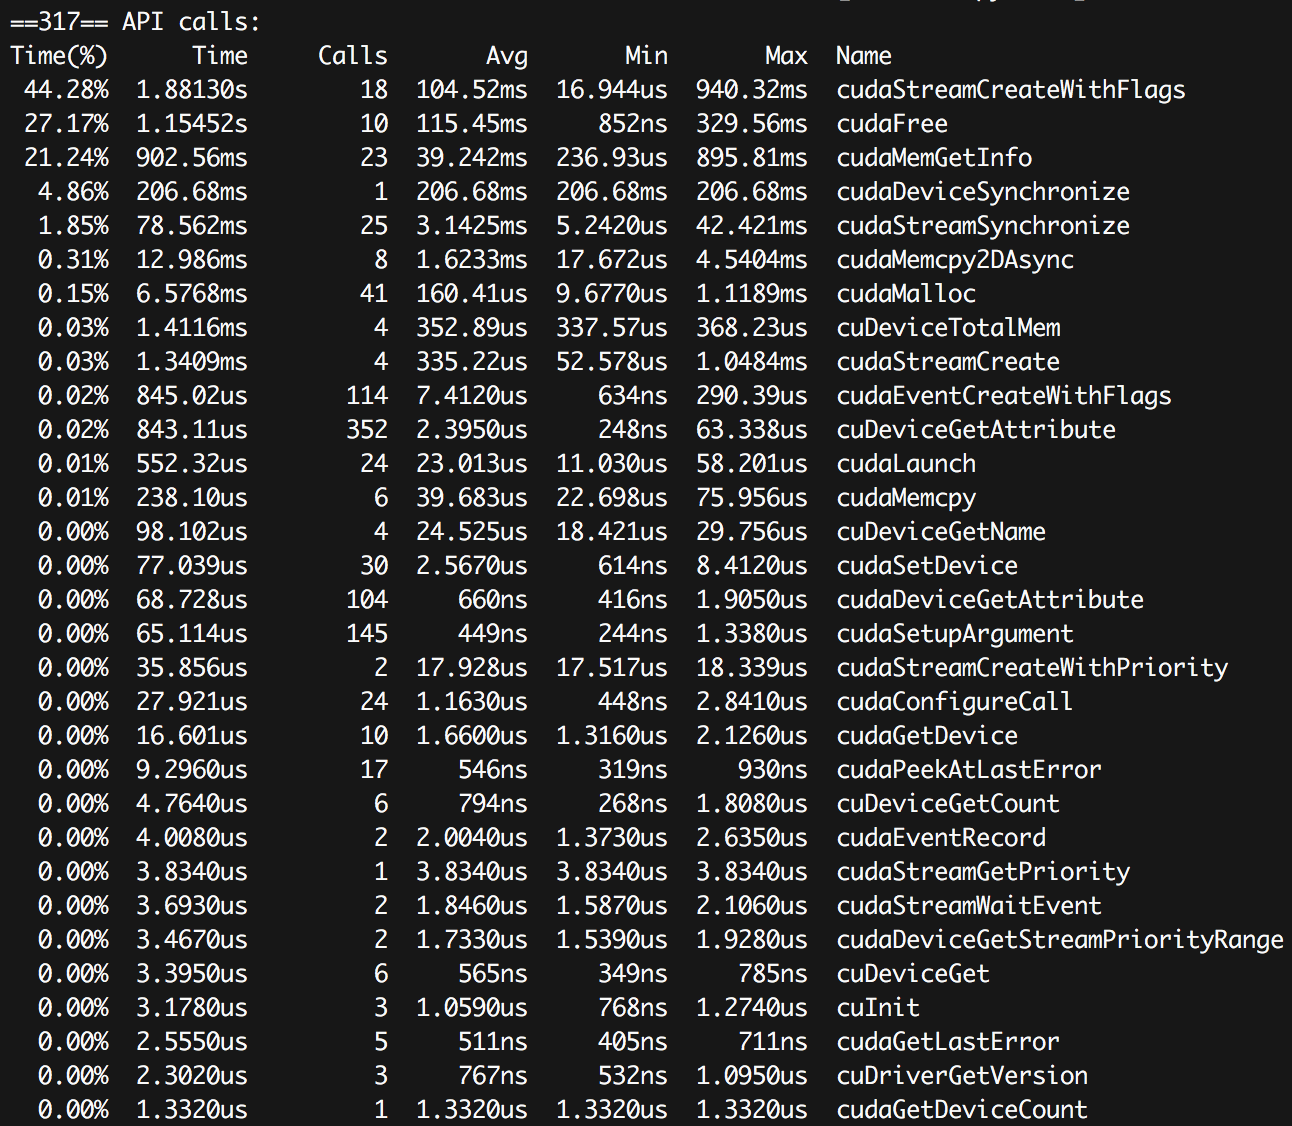
\includegraphics[width=\linewidth]{rai2.png}
\caption{Nvprof GPU profile for our optimized forward kernel}
\label{fig:flowFree}
\end{figure}

\newpage
\subsection*{Summary}
\noindent
From the profiler, we can see a heavy increase in runtime speed from the running time of our previous implementation in milestone 3, showing that the shared memory and tiling improvements we implemented were truly worthwhile, and effective in making our forward convolution kernel much faster than it previously was. This implementation was influenced by the implementation in the textbook, which served as a great model for implementing a tiling kernel that utilized the benefits of shared memory to achieve peak performance.


\section*{Team Contributions}
We all met up together and finished the sequential code for the convolutional layer in person. We also met up and wrote the parallel code together after 
meeting up in person, as well as crafting this report together for submission. Then for the final optimizations, we met up in person to speak about the implementation we were going to pursue, and used an online repository to assist each other in the implementation of our final kernel. We then documented our respective contributions in the report.

\end{document}















